
\documentclass{IOS-Book-Article}
\usepackage{graphicx}

\usepackage{float} % keeps tables in the exact position they occupy in the code
\usepackage{mathptmx}
\usepackage{soul}\setuldepth{article}
%\usepackage{times}
%\normalfont
%\usepackage[T1]{fontenc}
%\usepackage[mtplusscr,mtbold]{mathtime}
%
\def\hb{\hbox to 11.5 cm{}}

\begin{document}

\pagestyle{headings}
\def\thepage{}
\begin{frontmatter}              % The preamble begins here.


%\pretitle{Pretitle}
\title{Health-related content in transformer-based language models:\\ Bias in domain-specific training sets.}

\markboth{}{January 2023\hb}
%\subtitle{Subtitle}


\author[A]{\fnms{Caterina} \snm{Bonan}\orcid{0000-0002-4808-6865}%
}
and
\author[B]{\fnms{Giuseppe} \snm{Samo}\orcid{0000-0003-3449-8006}
\thanks{Corresponding Author: Giuseppe Samo, Department of Linguistics, University of Geneva, E-mail: giuseppe.samo@unige.ch; mail: Rue de Candolle 2, 1205 Geneva, Switzerland. }}
\runningauthor{Bonan \& Samo}
\address[A]{University of Cambridge}
\address[B]{University of Geneva}

\begin{abstract}
In this short communication, we implement and improve results from \cite{r1}, in which we claimed that the syntactic bias observed in general-purpose training sets urged the creation of domain-specific health-communication corpora, and predicted better performance for the latter. 
\end{abstract}

\begin{keyword}
Natural Language Processing\sep Health-content\sep 
Language Models\sep Knowledge Reproduction\sep Corpora\sep COVID-19
\end{keyword}
\end{frontmatter}
\markboth{January 2023\hb}{January 2023\hb}
%\thispagestyle{empty}
%\pagestyle{empty}

\section{Introduction}

%aggiungere articolo della Ettinger
Recent developments in Natural Language Processing have
demonstrated the ability of artificial neural language models in parsing and producing complex linguistic structures across languages (see [1] for an overview). Neural language models can be queried with naturally occurring sentences compared with minimally differing ex-novo examples, allowing us to elegantly detect and quantify asymmetries between pairs of isolated conditions.
In this contribution, we explore two languages and different training set to detect forms of bias in real-world representations with respect to medical semantic-encyclopedic knowledge adopting and improving the dataset discussed in [2], which tested and detected syntactic bias of transformer-based neural language models with respect to a list of mythbusters on COVID-19 extracted from a corpus the World Health Organization. We present a study below.\footnote{\footnote{Additional information with respect to the data are all available at the following link:}}

\section{The study}
\textbf{Hypothesis} In [2]'s conclusions, the authors aimed in future studies to detect whether the observed results was due to the type of investigated training data. Specifically, whether neural language models trained domain-specific datasets might perform better than those trained with domain-general data.

\noindent \textbf{Materials} The queried dataset is provided by the authors in [2] for English and Chinese. The training sets of languages of our contribution is presented in table \ref{models}.

\begin{table}[]
    \centering
    \begin{tabular}{l|l|l}
         \textsc{Language} & \textsc{Language Model} & \textsc{Training set type}\\ \hline
         English & \href{https://huggingface.co/docs/transformers/model_doc/bert}{\underline{BERT}} & Domain general (web, wiki)\\
         English & \href{https://huggingface.co/docs/transformers/model_doc/big_bird}{\underline{BigBird}} & Domain general (web, wiki)\\
         English & \href{https://huggingface.co/austinmw/distilbert-base-uncased-finetuned-health_facts}{\underline{HealthF}} & Domain specific (fact checking)\\
         English & \href{https://huggingface.co/publichealthsurveillance/PHS-BERT}{\underline{PHS}} & Domain specific (health surveillance on social media)\\
         Chinese & \href{https://huggingface.co/bert-base-chinese}{\underline{Bert}} & Domain general (web, wiki)\\
         Chinese & \href{https://huggingface.co/nghuyong/ernie-health-zh}{\underline{HealthZH}} & Domain specific (medical dialogues, records, textbooks)\\ \hline
    \end{tabular}
    \caption{Language Models used in this paper.}
    \label{models}
\end{table}

\noindent \textbf{Methods} The methodology is the one followed in [2]. The machine is presented with two sentences (i) a \textsc{true} statement extracted from the corpus and (ii) a \textsc{false} statement created with logical operators (see [2] for details). Our measure is the represented by the difference between the suprisal (the logarithm) of the \textsc{true} and the \textsc{false} statement. The higher the results the less performing (more surprisal for true sentences) the architectures.

\begin{figure}
    \centering
    \small
    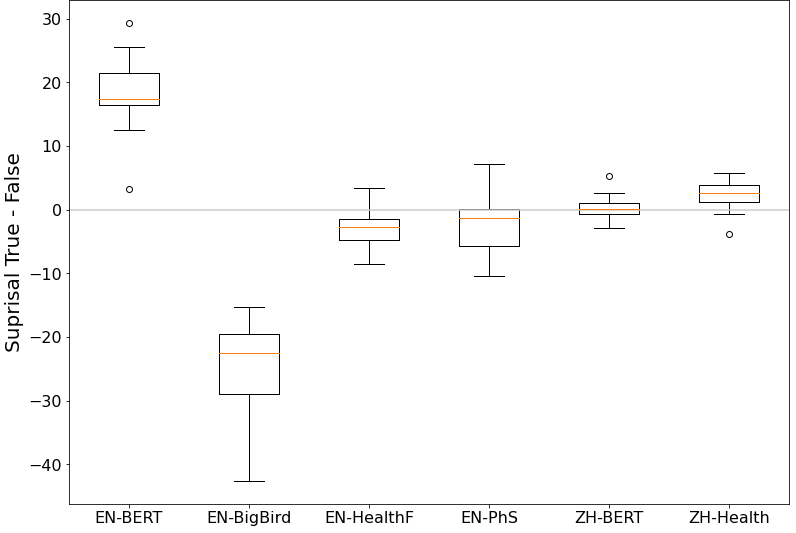
\includegraphics[scale=0.35]{graphmatplot}
    \caption{True-False across language models. }
    \label{fig:my_label}
\end{figure}

\noindent \textbf{Results} Our results are different across languages. We observe asymmetries: while one general-domain architecture perform worse BERT (M = 18.269, SD = 5.82 ) than domain-specific (\textit{F} (3, 64) = 177.30362; p $<$ .00001) but at the same time BigBird results in the best performance (M = -24.459, SD = 7.0771364), possibly due to sparse/global attention. In Chinese, the general domain performs ( \textit{M} = 0.510, \textit{SD} = 2.421) better than the domain-specific one ( \textit{M} = 1.81, \textit{SD} = 2.418) (\textit{t}(34) = 2.6837, p. $<$ .05).

\noindent \textbf{Conclusions and future studies}
In this paper, we provided a methodology to test bias of in multilingual corpora [3]

\begin{thebibliography}{99}


\bibitem{r1}
Linzen T, Baroni M. Syntactic Structure from Deep Learning. Annual Review of Linguistics 7:1,
Jan.2021;195-212.

\bibitem{r2}
Samo G, Bonan C, Si F. Health-Related Content in Transformer-Based Deep Neural Network Language Models: Exploring Cross-Linguistic Syntactic Bias. Stud Health Technol Inform. 2022 Jun 29;295:221-225. doi: 10.3233/SHTI220702. PMID: 35773848.

\bibitem{r3}
Utunen P, Ndiaye N, Attias M, Mattar L. Multilingual Approach to COVID-19 Online Learning
Response on OpenWHO.org. In: Mantas J, Hasman A, Househ MS, Gallos P, Zoulias E, Liaskos J,
editors. Informatics and Technology in Clinical Care and Public Health; IOS Press, 2022;Jan:192-5.

\end{thebibliography}
\end{document}
